\documentclass{standalone}
\usepackage{tikz}

\usetikzlibrary{shapes,arrows,fit,calc,positioning}
\usetikzlibrary{backgrounds}
\tikzstyle{box} = [draw, rectangle, fill=white, rounded corners, thick, node distance=5em, text width=7em, text centered, minimum height=2.5em]
\tikzstyle{container} = [draw, rectangle, dashed, inner sep=1em, node distance=5em]
\tikzstyle{line} = [draw, thick, -latex']
\begin{document}
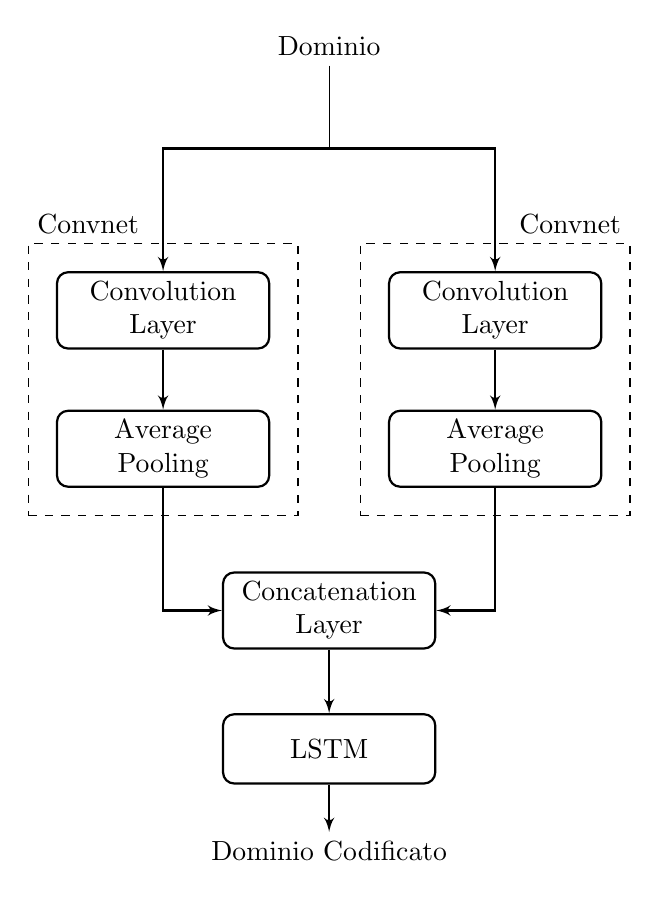
\begin{tikzpicture}[auto]
	\node [box] (conv) {Convolution Layer};
%	\node [box, below of=conv] (batch) {Batch Normalization};
%	\node [box, below of=batch](leaky) {Leaky ReLU activation};
%	\node [box, below of=leaky](dropout) {Dropout};
	\node [box, below of=conv](pooling){Average Pooling};

	\node [box, right of=conv, node distance=12em] (conv2) {Convolution Layer};
%	\node [box, below of=conv2] (batch2) {Batch Normalization};
%	\node [box, below of=batch2](leaky2) {Leaky ReLU activation};
%	\node [box, below of=leaky2](dropout2) {Dropout};
	\node [box, below of=conv2](pooling2){Average Pooling};
	
	\node [draw=none, above of=conv](invis4){};
	\node [draw=none, above of=conv2](invis5){};
	\node [draw=none, fit=(invis4)(invis5)](invis6){};
	\coordinate[above of=invis6,node distance=3em](begin_enc);
	\coordinate[above of=begin_enc,node distance=3em](in);
	\node at (begin_enc.north) [above,node distance=0 and 0] (input){};
	\node at (in.north) [above,node distance=0 and 0] (input){Dominio};

	\node [draw=none, below of=pooling](invis){};
	\node [draw=none, below of=pooling2](invis2){};
	\node [draw=none, fit=(invis)(invis2)](invis3){};
	
	\node[box,below of=invis3, node distance=3em](conc){Concatenation Layer};
	\node[box,below of=conc](lstm){LSTM};
	\coordinate[below of=lstm,node distance=3em](end_enc);
	\node at (end_enc.south) [below,node distance=0 and 0] (output){Dominio Codificato};

	\node [container, fit=(conv)(pooling)](cnn){};
	\node [container, fit=(conv2)(pooling2)](cnn2){};
	\node at (cnn.north west) [above right,node distance=0 and 0] {Convnet};
	\node at (cnn2.north east) [above left,node distance=0 and 0] {Convnet};

	\path [line] (conv) -- (pooling);
%	\path [line] (batch) -- (leaky);
%	\path [line] (leaky) -- (dropout);
%	\path [line] (dropout) -- (pooling);
	\path [line] (pooling) |- (conc);

	\path [line] (conv2) -- (pooling2);
%	\path [line] (batch2) -- (leaky2);
%	\path [line] (leaky2) -- (dropout2);
%	\path [line] (dropout2) -- (pooling2);
	\path [line] (pooling2) |- (conc);
	
	\path [line] (conc) -- (lstm);
	\path [line] (lstm) -- (end_enc);
	
	\draw (in) -- (begin_enc);
	\path [line] (begin_enc) -| (conv);
	\path [line] (begin_enc) -| (conv2);
\end{tikzpicture}
\end{document}